\section{Durchführung}
\label{sec:Durchführung}

Der Versuchsaufbau wird schematisch in \autoref{tab:3} dargestellt.\\
Zu erst werden die Spiegel so adjustiert, dass die Intensitätsmaxima sich auf dem Detektorschlitz überlagern und wenig Rillen zu sehen sind. \\
An einem Spiegel ist ein Motor angeschlossen, der dessen Position stetig verändert. Ein elektronisches Zählwerk misst die Lichtimpulse, die den Detektorschlitz erreichen. Nachdem die Schraube sich um 5 mm verschoben hat, werden die durch den Detektor gemessenen Impulse notiert und anhand dessen die Wellenlänge ermittelt.\\
Für den Brechungsindex wird mit einem Manometer die Luft innerhalb einer Zelle evakuiert oder ein Druck von 0.8 bar hinzugefügt. Die dadurch verursachten Interferenzen werden wieder mit einem elektronischen Zählwerk gezählt und die Impulse notiert.
\begin{figure}[H]
  \centering
  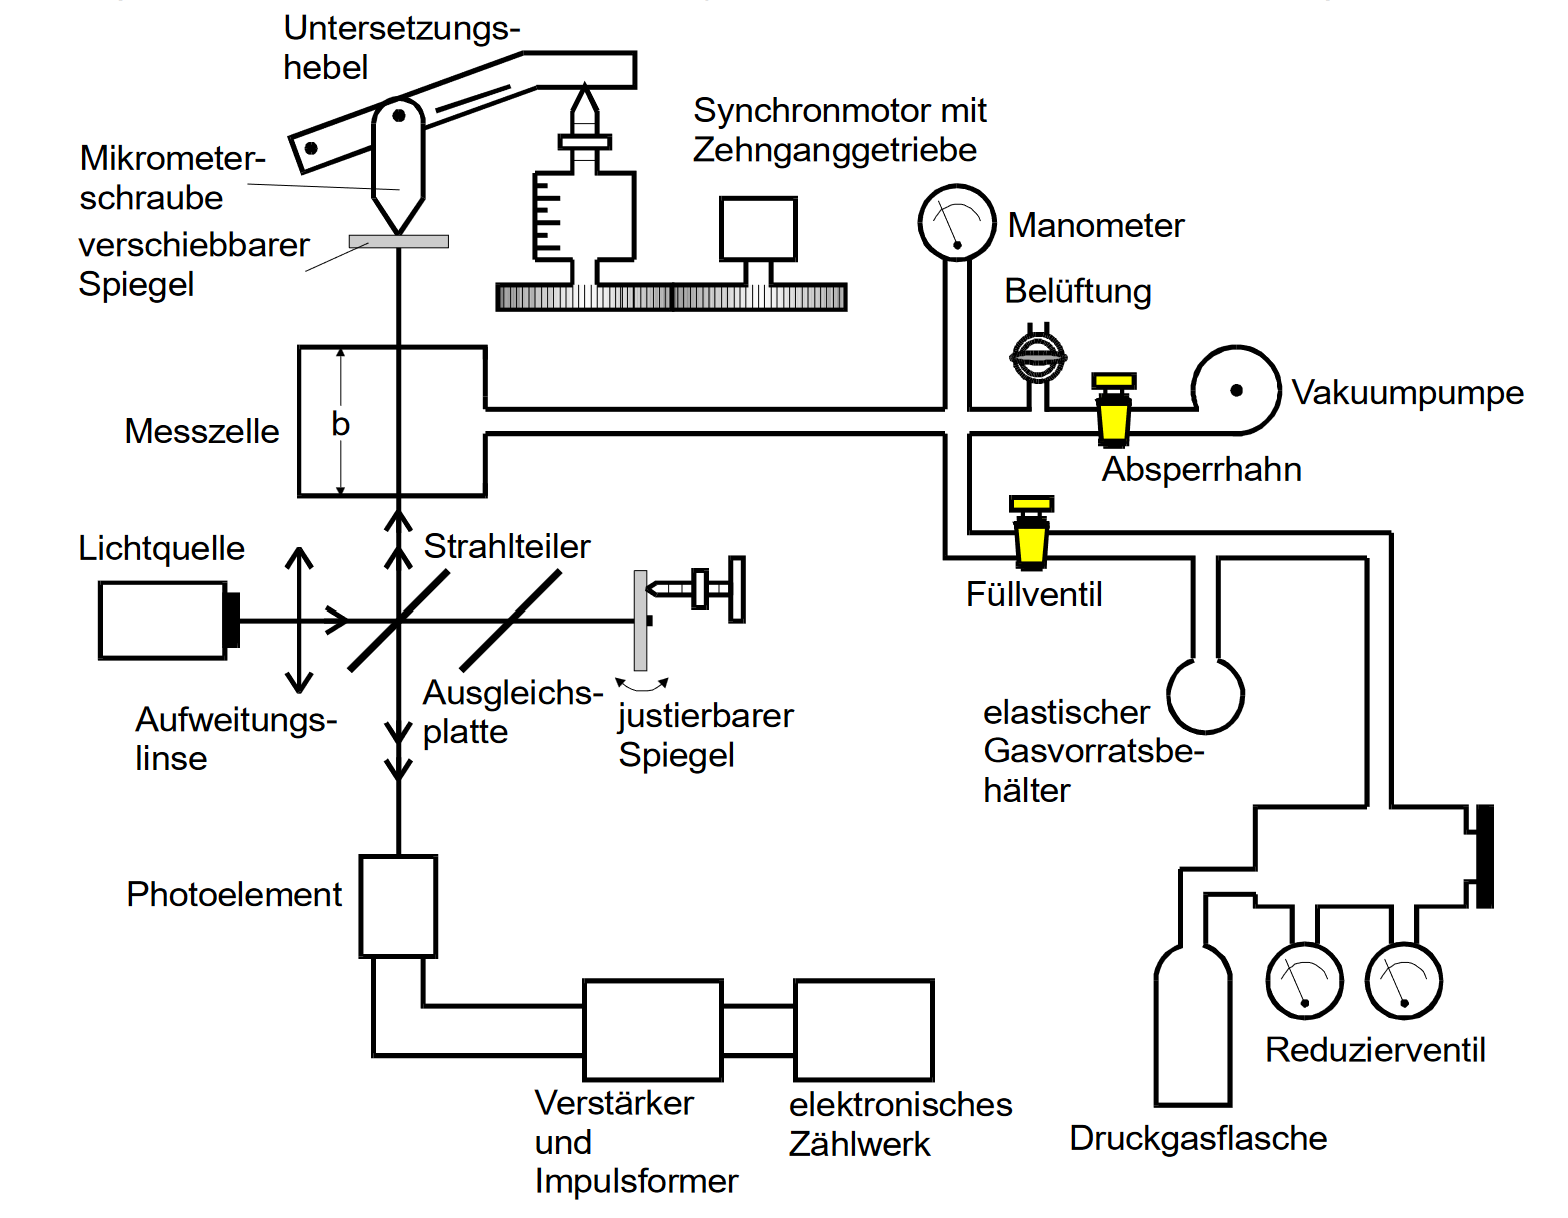
\includegraphics[width=9cm]{3.png}
  \caption{Schematischer Aufbau des Versuchs.}
  \label{tab:3}
\end{figure}
